% CVPR 2022 Paper Template
% based on the CVPR template provided by Ming-Ming Cheng (https://github.com/MCG-NKU/CVPR_Template)
% modified and extended by Stefan Roth (stefan.roth@NOSPAMtu-darmstadt.de)

\documentclass[10pt,twocolumn,letterpaper]{article}

%%%%%%%%% PAPER TYPE  - PLEASE UPDATE FOR FINAL VERSION %%%%%%%%%
%\usepackage[review]{cvpr}      % To produce the REVIEW version
%\usepackage{cvpr}              % To produce the CAMERA-READY version
\usepackage[pagenumbers]{cvpr} % To force page numbers, e.g. for an arXiv version

% Include other packages here, before hyperref.
\usepackage{graphicx}
\usepackage{amsmath}
\usepackage{amssymb}
\usepackage{booktabs}
\usepackage{float}
\usepackage[table,xcdraw]{xcolor}
\usepackage{arydshln}


% It is strongly recommended to use hyperref, especially for the review version.
% hyperref with option pagebackref eases the reviewers' job.
% Please disable hyperref *only* if you encounter grave issues, e.g. with the
% file validation for the camera-ready version.
%
% If you comment hyperref and then uncomment it, you should delete
% ReviewTempalte.aux before re-running LaTeX.
% (Or just hit 'q' on the first LaTeX run, let it finish, and you
%  should be clear).
\usepackage[pagebackref,breaklinks,colorlinks]{hyperref}


% Support for easy cross-referencing
\usepackage[capitalize]{cleveref}
\crefname{section}{Sec.}{Secs.}
\Crefname{section}{Section}{Sections}
\Crefname{table}{Table}{Tables}
\crefname{table}{Tab.}{Tabs.}

\begin{document}

%%%%%%%%% TITLE - PLEASE UPDATE %%%%%%%%%
\title{VRDL HW2: Digit Recognition Report}

\author{Yi-Hsiang Ho, 111550106
% For a paper whose authors are all at the same institution,
% omit the following lines up until the closing ``}''.
% Additional authors and addresses can be added with ``\and'',
% just like the second author.
% To save space, use either the email address or home page, not both
% \and
% Second Author\\
% Institution2\\
% First line of institution2 address\\
% {\tt\small secondauthor@i2.org}
}
\maketitle

%%%%%%%%% BODY TEXT %%%%%%%%%
\section{Introduction}
\label{sec:intro}

This task is to locate the digit in an image and recognize it using Faster
R-CNN. The core idea of this work is to leverage restart learning rate
scheduler and adjust anchor aspect and size. ResNet-101 is chosen to be the
backbone of the model. GitHub repository is available
\href{https://github.com/Sean20405/NYCU-DLVR-HW2}{here}.

%-------------------------------------------------------------------------

\subsection{Faster R-CNN}

Faster R-CNN is a widely used deep learning framework for object detection.
It builds upon earlier R-CNN models by integrating region proposal
generation and object classification into a single network, significantly
improving both speed and accuracy. The architecture consists of a
convolutional backbone for feature extraction, a Region Proposal Network
(RPN) that suggests potential object locations, and a head inherited from
Fast R-CNN that refines these proposals and classifies the objects. Unlike
its predecessors, Faster R-CNN eliminates the need for external region
proposal methods, such as selective search, by using the RPN to efficiently
generate high-quality proposals directly from the feature maps.~\cite{FasterRCNN}

\subsection{Region Proposal Network (RPN)}
The Region Proposal Network (RPN) is a key component of Faster R-CNN that
efficiently generates object proposals directly from feature maps produced
by the convolutional backbone. RPN slides a small network over the feature
map and predicts objectness scores and bounding box for multiple anchors.
These anchors vary in scale and aspect ratio, allowing the RPN to detect
objects of different shapes and sizes. By sharing convolutional features
with the detection network, the RPN significantly speeds up the proposal
process while maintaining high accuracy.

\subsection{Restart Learning Rate Scheduler}

Restart is a technique used in training neural networks to avoid local
minima by periodically resetting the learning rate. Instead of steadily
decreasing the learning rate throughout training, this approach reduces
it over time but then abruptly increases it at predefined intervals,
effectively restarting the optimization process. This strategy encourages
the model to explore new regions of the loss landscape after each restart,
often leading to better generalization.


\section{Method}
\label{sec:method}

\subsection{Model Architecture}

The backbone was changed from ResNet-50 (default) to ResNet-101 for a better
feature extraction. It is trained from the ImageNet pretrained Weights retrieved
from PyTorch as \verb'ResNet101_Weights.IMAGENET1K_V2'. 

The architecture of RPN doesn't change. But the anchor size and aspect ratio
are adjusted to fit this task. Since digits are usually small and rectangular,
the anchor size is set from 16x16 to 256x256 and the aspect ratio is set to
1:4, 1:2, 1:1, 2:1, and 4:1. There are 25 anchors in total. This allows the
model to better capture the bounding boxes of digits.~\cite{TorchVision}

After region proposals are generated and refined (by NMS) by RPN, they are
projected onto the shared feature map and passed through a RoI pooling to
produce fixed-size feature vectors. These vectors are then fed into 2 layers
of MLP and 1 branched MLP to output classification and bounding box regression.
This part keeps the same as the initial implementation.

\subsection{Optimization}

For optimization, AdamW is used with an initial learning rate of 5e-5. A
cosine annealing scheduler dynamically adjusts the learning rate throughout
training. A restart strategy is adopted to avoid local minima. It will restart
after the first 10,000 steps, and the number of steps between each restart
will double. That is, the next restart will occur after the next 20,000 steps,
which is at step 30,000. Since the total number of steps is about 70,000,
it will restart three times. \cref{fig:restart} visualizes the
change of the learning rate.

Training process is performed with a batch size of 8 over 20 epochs. The
provided dataset contains roughly 30,000 training images, 3,000 validation
images, and 13,000 test images. The best-performing model is selected based
on the validation accuracy. The model is trained on a single NVIDIA GeForce
RTX 4090 GPU in about 8.5 hours.

\subsection{Inference}

During inference, an image will be fed into the model to generate labels,
bounding boxes and the confidence score. The boxes with score lower than 0.5
will be discarded. The remaining boxes will be involved in the final number
prediction. The final prediction is based on the location of the bounding
box. Sort the boxes in one image from left to right, top to bottom, and
concatenate the label for the sorted boxes. The final result is a string of
digits like "123".

\begin{figure}[h]
  \centering
  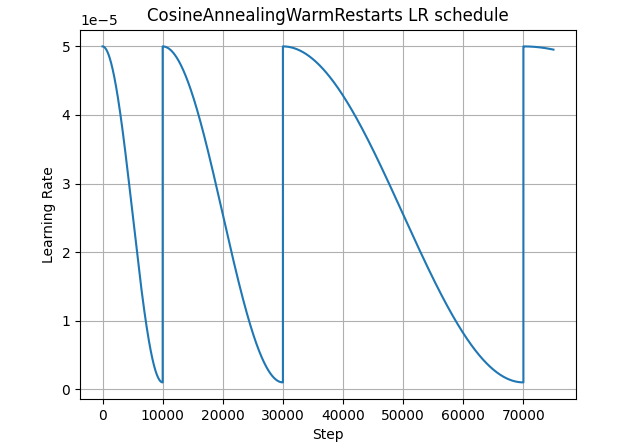
\includegraphics[width=0.8\linewidth]{assets/restart.png}
  \caption{\textbf{Visualization of restart learning rate scheduler.} The learning rate
    is reduced over time but then abruptly increased at predefined intervals.}
  \label{fig:restart}
\end{figure}

\subsection{Hyperparameters}

\noindent The hyperparameter details are listed below:
\begin{itemize}
  \setlength\itemsep{0pt}
  \item Learning rate: 5e-5
  \item Optimizer: AdamW
  \item Scheduler: CosineAnnealingWarmRestarts ($T_0=10,000,\ T_{\text{mul}}=2$)
  \item Batch Size: 16
  \item Epochs: 20
  \item Anchor size: 16x16, 32x32, 64x64, 128x128, 256x256
  \item Anchor aspect: 0.25 (1:4), 0.5 (1:2), 1.0 (1:1), 2.0 (2:1), 4.0 (4:1)
\end{itemize}

\section{Results}

In this section, I compare the performance of each component in the model.
The details of each method are listed:
\begin{itemize}
  \setlength\itemsep{0pt}
  \item Res101: ResNet 101 pretrained on ImageNet without any tricks.
  \item Restart: Res101 with restart learning rate scheduler.
  \item Anchor: Change anchor size and aspect ratio.
  \item All: Combines all the techniques mentioned in \cref{sec:method}.
\end{itemize}

The validation accuracy is calculated by comparing the final result of the model and
the ground truth for each image. The ground truth labels and boxes are converted to
a string of digits using the same method mentioned above. While the mAP is calculated
per boxes and labels between the predicted and ground truth. The mAP is calculated as
average AP at each IoU threshold, from 0.5 to 0.95 with a step of 0.05, and each label.

The results are shown in \cref{tab:result-acc} and \cref{tab:result-map}. All the results here
are evaluated by choosing the best checkpoint based on the validation accuracy. Using
customized anchors shows a great improvement in the accuracy while the restart strategy
improves the mAP much. The combination of all the techniques achieves the best performance.

\begin{table}[h]
  \centering
  \begin{tabular}{lccc}
    \toprule
    \multicolumn{1}{c}{\textbf{Method}} & \textbf{Val}    & \textbf{Test pub.} & \textbf{Test priv.} \\
    \midrule
    Res101                              & 0.8063          & 0.7536             & 0.7557              \\
    Restart                             & 0.8045          & 0.7580             & 0.7564              \\
    Anchor                              & 0.8168          & 0.7777             & 0.7727              \\
    All                                 & \textbf{0.8177} & \textbf{0.7840}    & \textbf{0.7810}     \\
    \bottomrule
  \end{tabular}
  \caption{\textbf{Accuracy results of different models.} "Val" refers to
    validation accuracy. "Test pub." and "Test priv." refer to public and
    private test set accuracy, respectively. The highestv values in each
    column are highlighted in bold.
  }
  \label{tab:result-acc}
\end{table}

\begin{table}[h]
  \centering
  \begin{tabular}{lccc}
    \toprule
    \multicolumn{1}{c}{\textbf{Method}} & \textbf{Val}    & \textbf{Test pub.} & \textbf{Test priv.} \\
    \midrule
    Res101                              & 0.4526          & 0.3686             & 0.3681              \\
    Restart                             & 0.4554          & \textbf{0.3770}    & \textbf{0.3777}     \\
    Anchor                              & 0.4524          & 0.3720             & 0.3706              \\
    All                                 & \textbf{0.4581} & 0.3751             & \textbf{0.3777}     \\
    \bottomrule
  \end{tabular}
  \caption{\textbf{mAP results of different models.} The definition of the
    term is the same as \cref{tab:result-acc}. The highestv values in each
    column are highlighted in bold.
  }
  \label{tab:result-map}
\end{table}

The validation accuracy, mAP and training loss curve are shown in \cref{fig:val-acc},
\cref{fig:val-mAP} and \cref{fig:train-loss}, respectively. At first, I found that Res101 has a
very steady training process. The accuracy and mAP keep increasing, the loss keeps
decreasing, and it converges quickly. Thus, I plan to use restart strategy to add
some interference in the training process. The restart strategy works well. While
a restart happens (roughly at epoch 2, 7, and 18), the accuracy and mAP drop a little
but then increase rapidly. The training loss also rises after each restart. This indicates
that the model is exploring new regions of the loss landscape.

\begin{figure}[h]
  \centering
  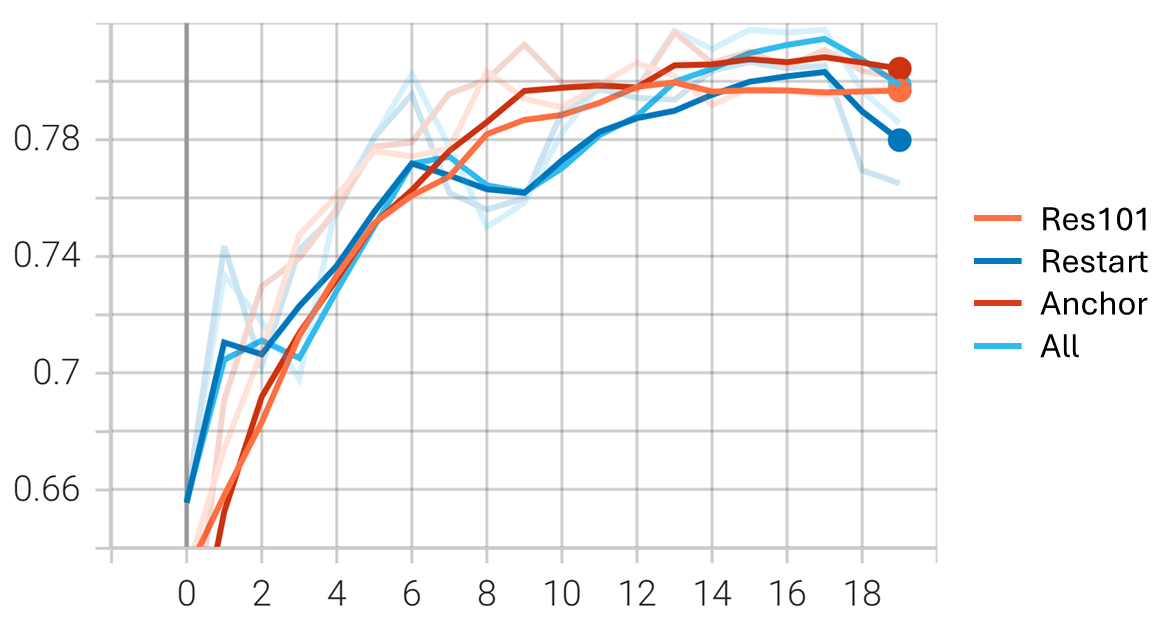
\includegraphics[width=0.9\linewidth]{assets/val_acc.png}
  \caption{\textbf{Validation accuracy curve.}}
  \label{fig:val-acc}
\end{figure}

\begin{figure}[h]
  \centering
  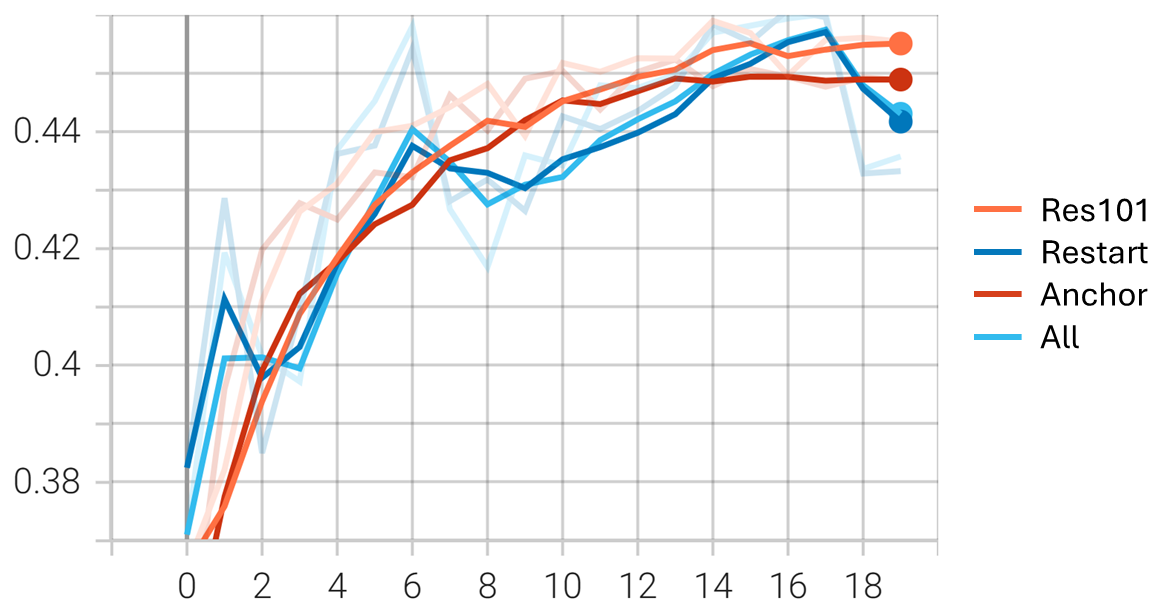
\includegraphics[width=0.9\linewidth]{assets/val_mAP.png}
  \caption{\textbf{Validation mAP curve.}}
  \label{fig:val-mAP}
\end{figure}

\begin{figure}[h]
  \centering
  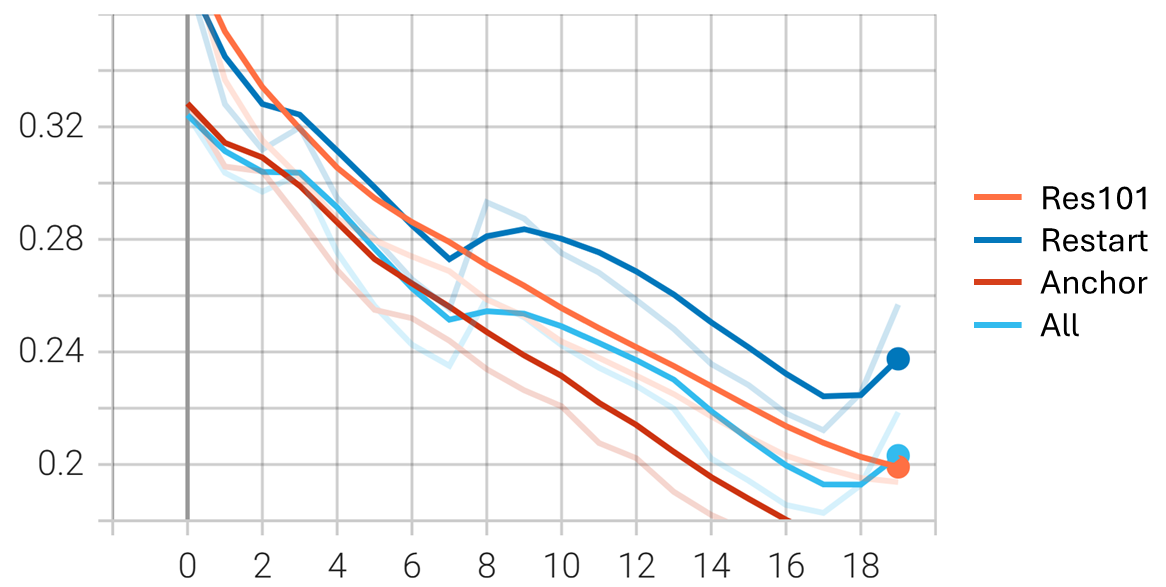
\includegraphics[width=0.9\linewidth]{assets/train_loss.png}
  \caption{\textbf{Training loss curve.}}
  \label{fig:train-loss}
\end{figure}

\section*{Other Experiments}

\subsection*{The Selection of Best Checkpoint}

The best checkpoint is selected based on the validation accuracy. I've
also tried to select based on the mAP. However, the
mAP is not a good indicator of the model's performance. The mAP is
calculated based on the predicted boxes and labels. However, the
predicted boxes are not always accurate. The mAP is not sensitive to
the accuracy of the predicted boxes. Therefore, I choose to select
the best checkpoint based on the validation accuracy. \cref{tab:best-select}
verify this thought.

\begin{table}[h]
  \centering
  \setlength{\tabcolsep}{3.5pt}
  \begin{tabular}{lcccccc}
    \toprule
                                        & \multicolumn{3}{c}{\textbf{Accuracy}}            & \multicolumn{3}{c}{\textbf{mAP}}                 \\
    \cmidrule[0.3pt](lr){2-4} \cmidrule(lr){5-7}
    \multicolumn{1}{c}{\textbf{Method}} & \textbf{Val}   & \textbf{Pub.}  & \textbf{Priv.} & \textbf{Val}   & \textbf{Pub.}  & \textbf{Priv.} \\
    \midrule
    Res101 acc.                         & \textbf{0.806} & \textbf{0.754} & \textbf{0.756} & 0.453          & \textbf{0.369} & 0.368          \\
    Res101 mAP                          & 0.792          & 0.722          & 0.720          & \textbf{0.459} & 0.367          & \textbf{0.370} \\
    \midrule
    Restart acc.                        & \textbf{0.807} & \textbf{0.767} & \textbf{0.765} & 0.455          & \textbf{0.377} & \textbf{0.378} \\
    Restart mAP                         & 0.805          & 0.758          & 0.756          & \textbf{0.461} & 0.376          & 0.377          \\
    \bottomrule
  \end{tabular}
  \caption{\textbf{The result using different selection method.} "acc." 
    means the result of selecting the best checkpoint based on the validation
    accuracy, while "mAP" selects based on the mAP. The higher values are
    highlighted in bold. "Pub" is the same as "Test pub." in previous section,
    as well as "Priv."
  }
  \label{tab:best-select}
\end{table}

\subsection*{The Selection of Backbone}

The selection of the convolutional backbone may affect the model's performance.
I've conducted experiments with different backbones, ResNet50, ResNet101,
ResNeXt50 and ResNeXt101~\cite{ResNeXt}. The results are shown in \cref{tab:backbone-exp}.
Both ResNet101 and ResNeXt101 perform well, but ResNeXt101 has a poor performance
when integrating restart and anchor trick. It also needs 1.7x longer time to train
than ResNet101. Therefore, I choose ResNet101 as the backbone of the model.

\begin{table}[h]
  \centering
  \setlength{\tabcolsep}{3.5pt}
  \begin{tabular}{lcccccc}
    \toprule
                                        & \multicolumn{3}{c}{\textbf{Accuracy}}            & \multicolumn{3}{c}{\textbf{mAP}}                 \\
    \cmidrule[0.3pt](lr){2-4} \cmidrule(lr){5-7}
    \multicolumn{1}{c}{\textbf{Method}} & \textbf{Val}   & \textbf{Pub.}  & \textbf{Priv.} & \textbf{Val}   & \textbf{Pub.}  & \textbf{Priv.} \\
    \midrule
    ResNet50                            & 0.675          & 0.661          & 0.657          & 0.426          & 0.361          & 0.360          \\
    ResNet101                           & 0.806          & 0.754          & 0.756          & \textbf{0.453} & \textbf{0.369} & \textbf{0.368} \\
    ResNeXt50                           & 0.746          & 0.680          & 0.690          & 0.448          & 0.356          & 0.359          \\
    ResNeXt101                          & \textbf{0.808} & \textbf{0.757} & \textbf{0.761} & 0.450          & 0.365          & 0.366          \\
    \bottomrule
  \end{tabular}
  \caption{\textbf{The result of different backbone.} The highest values
    for each column are highlighted in bold.
  }
  \label{tab:backbone-exp}
\end{table}

\subsection*{Sharpening}

I've also experimented with shaprening the input image. I found
that the input image may be too blurred to recognize even by
human. Therefore, I tried to sharpen the image before passing it
to the model. It is implemented by PIL package. However it does
not consistently improve performance. The results are shown in
\cref{tab:sharp}. Thus, it is not included in the final model.

\begin{table}[h]
  \centering
  \setlength{\tabcolsep}{3.5pt}
  \begin{tabular}{lcccccc}
    \toprule
                                        & \multicolumn{3}{c}{\textbf{Accuracy}}            & \multicolumn{3}{c}{\textbf{mAP}}                 \\
    \cmidrule[0.3pt](lr){2-4} \cmidrule(lr){5-7}
    \multicolumn{1}{c}{\textbf{Method}} & \textbf{Val}   & \textbf{Pub.}  & \textbf{Priv.} & \textbf{Val}   & \textbf{Pub.}  & \textbf{Priv.} \\
    \midrule
    ResNet101                           & \textbf{0.806} & \textbf{0.754} & \textbf{0.756} & 0.453          & \textbf{0.369} & \textbf{0.368} \\
    ResNet101*                          & 0.796          & 0.733          & 0.740          & \textbf{0.457} & 0.367          & 0.367          \\
    \midrule
    Restart                             & 0.807          & 0.767          & 0.765          & 0.455          & \textbf{0.377} & \textbf{0.378} \\
    Restart*                            & \textbf{0.808} & \textbf{0.770} & \textbf{0.771} & \textbf{0.457} & 0.373          & 0.377          \\
    \midrule
    All                                 & \textbf{0.818} & 0.784          & 0.781          & \textbf{0.458} & \textbf{0.375} & \textbf{0.378} \\
    All*                                & 0.814          & \textbf{0.786} & \textbf{0.786} & 0.451          & 0.374          & 0.371          \\
    \bottomrule
  \end{tabular}
  \caption{\textbf{The result of adding sharpening.} The higher values
    for each column are highlighted in bold. * means adding sharpening.
  }
  \label{tab:sharp}
\end{table}

%%%%%%%%% REFERENCES %%%%%%%%%
{\small
\bibliographystyle{ieee_fullname}
\bibliography{egbib}
}

\end{document}